\setcounter{chapter}{10-1} %Makes the prereq chapter chapter 0

\chapter{Optimizing Neural Networks}

    These notes carry over from the \vocab{Neural Networks} chapter. Here, we include topics that we previously skimmed over.

    \section{Strategies towards adaptive step-size}

        \subsection{Momentum}
    
        \subsubsection{Solving Oscillation}
    
            Let's look at one common problem we have with gradient descent: \textbf{oscillation}. 
            
            \begin{figure}[H]
                \centering
                    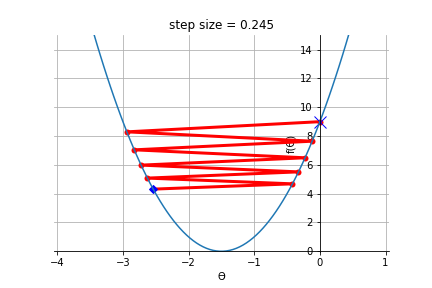
\includegraphics[width=70mm,scale=0.5]{images/gradient_descent_images/oscillate.png}
            \end{figure}
            
            We overshoot our target, and then have to take another step that \textbf{undoes} most of what happened in the previous step. So, we waste a lot of time correcting the last step.
                \note{For example, our first two steps land us in almost the same place we started!}
                
            This can significantly \textbf{slow} down how quickly we converge.
                
            \begin{figure}[H]
                \centering
                    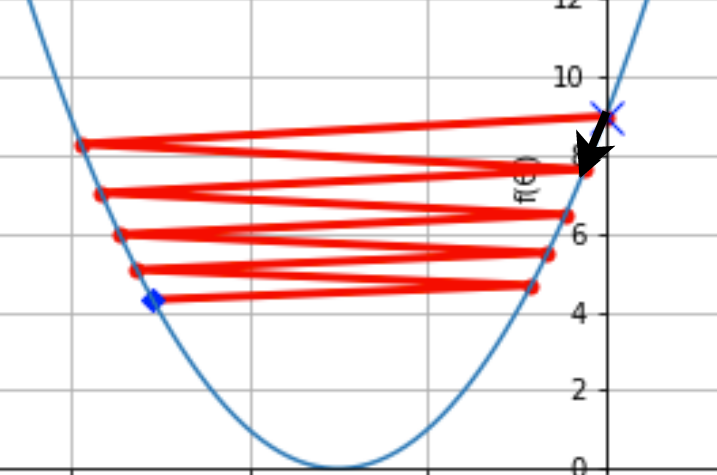
\includegraphics[width=70mm,scale=0.5]{images/nn_2_images/oscillate_zoom.png}
                
                \caption*{The black arrow shows the combined effect of our first two steps: almost nothing!}
            \end{figure}
            
            We don't want to waste time, so we want to remove the "part" of the gradient that is likely to \textbf{cancel} out. 
            
            The \textbf{next} gradient cancels out some of the previous. Our first two steps add up, or "\textbf{average} out" to a small improvement.
            
            If our steps are effectively "averaging", we'll speed up that process: we'll average together the gradients \textit{before} taking our step!
                \note{This means we can take a bigger step in a direction we won't have to cancel!}\\
                
            \begin{concept}
                Since our gradient descent steps \gren{combine} to give us our new model, we can think of them as adding, or "\purp{averaging}" to a more accurate improvement.
            \end{concept}
            
                \note{The only real difference between adding and averaging is whether we divide by the number of terms.}
            
            When our function \textbf{oscillates}, we get the same pattern \textbf{multiple} times: past steps indicate the sort of pattern we'll see in \textbf{future} steps. 
            
            So, we'll average our current gradient with past gradients: that way, the \textbf{component} that gets cancelled out is \textbf{removed}, and we won't have to undo our mistake over and over.\\
            
            \begin{concept}
                \vocab{Oscillation} causes us to move back and forth over the same region \purp{multiple} times, where each step mostly \gren{cancels} out the last.
                
                One solution is to \purp{average out} multiple of our gradients: the part that is "\gren{cancelled} out" should be eliminated by the average.
                
                So, we average our \gren{past} gradients (past oscillation) with our \gren{current} gradient, so we move in a more \purp{efficient} direction, speeding up our algorithm.
            \end{concept}
            
            Another way to think about it: when we \textbf{average} out our current and previous gradient, we're cancelling out what they "\textbf{disagree}" on, and keeping what they \textbf{agree} on.
            
            So, we're taking a step in the direction that multiple gradients agree will \textbf{improve} our model!
            
        
        \phantom{}
            
        \subsubsection{Weighted averages}
        
            We could naively average all of our gradients \gren{equally}. But, this would be a bad idea:
            
            \begin{itemize}
                \item It doesn't give you as much control of the algorithm: what if we care more about the \textbf{present} gradient, than the previous one?
                \item Gradients further in the \purp{past} are \textbf{less likely} to matter: we've moved further away from those positions.
                    \begin{itemize}
                        \item We also need to \textbf{scale} down past terms, so they don't take up most of the average.
                            \note{If you're averaging 100 terms, and you add one more... it's not going to change much.}
                    \end{itemize}
            \end{itemize}
            
            The first problem is easy to solve: we'll \textbf{weigh} each of our terms differently.\\
            
            \begin{concept}
                A \vocab{weighted average} is used when we want some terms to affect our \purp{average} more than others.
                
                We represent this with \gren{weights}: each weight represents the \purp{proportion} of our average from that term.
                
                \begin{equation*}
                    \text{Weighted Average} =
                    x_1w_1 + x_2w_2 + \dots + x_nw_n
                \end{equation*}
            \end{concept}

                \note{These weights are \orgg{separate} from the weights inside our neural network.

                \phantom{}
                
                They do, however, represent the same type of concept: the NN weights scale the \gren{input}, while these weights scale the \purp{gradients}.}
            
            \miniex If $w_1=\red{.6}$, that means \red{60\%} of the average comes from $x_1$.
            
            Note that, since we're talking about \textbf{proportions}, they need to \orgg{sum to 1}: it wouldn't make sense to have more than 100\% of the average.
            
            At each time step, we're adding one new gradient: the \textbf{present} one.
            
            We'll simplify our average to those two terms: the \textbf{present} gradient, versus all the \textbf{past} gradients.
            
            \begin{itemize}
                \item We represent the importance (\textbf{weight}) of our \redd{past} gradients using the variable $\red{\gamma}$.
                
                \item We want the two terms to add to 1: so, the importance of \vocab{current} gradient is $\blu{1-\gamma}$.
            \end{itemize}
            
            \begin{equation}
                \overbrace{
                    A_t 
                }^{\text{Average}}
                =
                \overbrace{
                    \red{\gamma} G_{t-1}
                }^{\text{Old gradients}}
                + \;\;
                \overbrace{
                    \blu{(1-\gamma)} g_{t}
                }^{\text{New gradient}}
            \end{equation}
            
            Now, we have \textbf{control} over how much the present or past gradient matters: we just have to adjust $\gamma$. 
            
        \phantom{}
        
        \subsubsection{Running Average}
        
            We still have some work to do: first, we haven't made it clear how we're incorporating our old gradients: we lumped them into one term.
            
            Let's try building up from $t=1$. We'll assume our previous gradients are 0, for simplicity.
            
            \begin{equation}
                A_0=g_0=0
            \end{equation}
            
            Our first step will average this with our \textbf{first} gradient:
            
            \begin{equation}
                A_1 
                =  
                \red{\gamma} g_0 \;\;+\;\; \blu{(1-\gamma)} g_1
            \end{equation}
            
            Simplifying to:
            
            \begin{equation}
                A_1 =  \blu{(1-\gamma)} g_1
            \end{equation}
            
            What about our second step? 
            
            \begin{equation}
                A_2
                =
                \overbrace{
                    \red{\gamma} G_{t-1}
                }^{\text{Old gradients}}
                + \;\;
                \blu{(1-\gamma)} g_2
            \end{equation}
            
            We \textit{could} just plug in $g_1$. But, $A_1$ contains the information about our first gradient $g_1$, \textbf{and} the gradient before it, $g_0$.
            
            \begin{equation}
                A_2
                =
                \overbrace{
                    \red{\gamma} A_1
                }^{\text{Contains $g_1$, $g_0$}}
                + \;\;
                \blu{(1-\gamma)} g_2
            \end{equation}
            
            We can repeat this process:
            
            \begin{equation}
                A_3 = 
                \overbrace{
                    \red{\gamma} A_{2}
                }^{\text{Contains $g_2$,$g_1$, $g_0$}}
                + \;\;
                \overbrace{
                    \blu{(1-\gamma)} g_3
                }^{\text{New gradient}}
            \end{equation}

            And so, we've created a general way to \textbf{average} as our program \textbf{runs} through different gradients.

            \begin{equation}
                A_t \;\;=\;\; 
                \gamma A_{t-1} \;\;+\;\; 
                (1-\gamma) g_t
            \end{equation}

            To allow more flexibility, we'll allow $\gamma$ to \orgg{vary in time}, as $\gamma_t$.
            
            \begin{equation}
                A_t \;\;=\;\; 
                \org{\gamma_t} A_{t-1} \;\;+\;\; 
                (1-\org{\gamma_t}) a_t
            \end{equation}

            \begin{itemize}
                \item We call this a \textbf{running average}.\\
            \end{itemize}

            \begin{definition}
                A \vocab{running average} is a way to average past data with present data \purp{smoothly}.

                Our \gren{initial} value for the average is typically zero:

                \begin{equation*}
                    A_0=0
                \end{equation*}

                Then, we begin introducing \orgg{new} data points.
                
                \begin{itemize}
                    \item You use the parameter $\gamma_t$ to indicate how much you want to prioritize \gren{past data}.
                    \item Thus, $1-\gamma_t$ indicates the value of \purp{new data}.
                \end{itemize}

                \begin{equation*}
                    \overbrace{
                        A_t 
                    }^{\text{Average}}
                    \;\;=\;\;
                    \overbrace{
                        \red{\gamma_t} A_{t-1}
                    }^{\text{Old gradients}}
                    \;\;+\;\; 
                    \overbrace{
                        \blu{(1-\gamma_t)} g_{t}
                    }^{\text{New gradient}}
                \end{equation*}

                \phantom{}

                \begin{itemize}
                    \item Note that instead of $\gamma$, we write $\gamma_t$: this "discount factor" can vary with time.

                \end{itemize}

                
            \end{definition}

            \phantom{}

            \begin{clarification}
                This is technically only one kind of \orgg{running average}: here, we use an "\vocab{exponential moving average}". 

                There are different ways to average past data points, with different \purp{weighting} schemes.
                    
                    \begin{itemize}
                        \item For example, you could do a "\gren{simple moving average}", where you average equally over the last $n$ data points.
                    \end{itemize}
            \end{clarification}

        \phantom{}

        \subsubsection{Running Averages: The Distant Past}

            So, how does this "running average" approach affect our different data points, further in the past? Let's find out.

            \phantom{}

            For simplicity, let's assume $\gamma_t=\gamma$: it's a \gren{constant}.

            \begin{equation}
                A_t 
                =
                \red{\gamma} \grn{A_{t-1}}
                + 
                \blu{(1-\gamma)} g_{t}
            \end{equation}

            We can expand $A_{t-1}$ to see further in the past:

            \begin{equation}
                A_t 
                =
                \red{\gamma} 
                    \Big(\red{\gamma} \grn{A_{t-2}}
                    + 
                    \blu{(1-\gamma)} g_{t-1}
                \Big)
                + 
                \blu{(1-\gamma)} g_{t}
            \end{equation}

            And even further: 
                \note{This is starting to get messy: don't worry if it's hard to read.}
            

            \begin{equation}
                A_t 
                =
                \red{\gamma} 
                \Bigg(\red{\gamma} 
                    \Big(
                        \red{\gamma} \grn{A_{t-3}}
                        + 
                        \blu{(1-\gamma)} g_{t-2}
                    \Big)
                    + 
                    \blu{(1-\gamma)} g_{t-1}
                \Bigg)
                + 
                \blu{(1-\gamma)} g_{t}
            \end{equation}

            Let's rewrite this.

            \begin{equation}
                \red{\gamma}^3 \grn{A_{t-3}}  \;\;+\;\; 
                \red{\gamma}^2\blu{(1-\gamma)} g_{t-2} \;\;+\;\;
                \red{\gamma}\blu{(1-\gamma)} g_{t-1} \;\;+\;\; 
                \blu{(1-\gamma)} g_{t}
            \end{equation}

            \phantom{}

            We see a "stacking" effect for $\gamma$: 
            
            \begin{itemize}
                \item We only partly include our newest data point: we scale it by $1-\gamma$, to make room for the past.

                \begin{equation}
                    \blu{(1-\gamma)} g_{t}
                \end{equation}
                
                \item But if your gradient is 1 time unit in the past, we apply $\gamma$ \orgg{once}, "forgetting" some more of that gradient.

                \begin{equation}
                    \red{\gamma}\blu{(1-\gamma)} g_{t-1}
                \end{equation}

                \item But if your gradient is 2 units in the past, we apply $\gamma$ \orgg{twice}: we've "forgotten" some of it twice.

                \begin{equation}
                    \red{\gamma}^2\blu{(1-\gamma)} g_{t-2}
                \end{equation}
            \end{itemize}

            Each time we do an average, we scale down our older data points by $\gamma$. So, the further in the past, the less effect they have.

            \begin{itemize}
                \item This is exactly the kind of design we wanted!\\
            \end{itemize}

            \begin{concept}
                A \purp{running average} tends to pay less attention to data further in the \gren{past}.

                \begin{itemize}
                    \item In general, if you are $k$ time units in the past, we apply a factor of \red{$\gamma^k$}.
                \end{itemize}

                Because $\gamma<1$, this \orgg{exponentially} decays to 0.

                \phantom{}

                If we want to fully expand $A_t$, it's easiest to use a sum:

                \begin{equation*}
                    A_T = \sum_{t=0}^T \red{\gamma^{(T-t)}} \cdot \blu{(1-\gamma)} \cdot g_t
                \end{equation*}
            \end{concept}
            You can compare this formulation against what we computed above.

            \phantom{}
            

        \subsubsection{Momentum}

            Applying a running average to our gradients gives us \purp{momentum}.

            \begin{itemize}
                \item This analogy to \textbf{physics} represents how our point "moves" through the \purp{weight space}, to optimize $J$.
                    \note{Gradient descent adjusts our weights: we go from one list of weights, to another. That's why we say we're moving through the "weight space".

                    \phantom{}
                    
                    Because our hypothesis is determined by our weights, this is also a "hypothesis space".}
                    
                \item The gradient gives us a "direction" of motion. So, our \gren{momentum} represents the direction we were "already moving": the \gren{previous} averaged gradient.
            \end{itemize}

            We use $M$ to represent the "averaged gradient" that we use to move. Our initial momentum is 0:

            \begin{equation}
                M_0=0
            \end{equation}

            And we want to average our current gradient with past gradients:

            \begin{equation}
                M_t 
                \;\;=\;\;
                \red{\gamma} \grn{M_{t-1}}
                \;\;+\;\; 
                \blu{(1-\gamma)} g_{t}
            \end{equation}

            What is our \purp{past} gradient $g_t$? Well, we want to use $W$ to modify $J$: $\pderiv{J}{W}$, or $\nabla_W J$.

            And we're moving through the \gren{weight space}, so our input to the gradient is the previous set of weights, $W_{t-1}$.

            \begin{equation}
                g_{t} = \nabla_W J (W_{t-1})
            \end{equation}

            And finally, $M_t$, our "averaged gradient", determines how we move.

            \begin{equation}
                W_t \;\;=\;\; W_{t-1} \;\;-\;\; \eta M_t
            \end{equation}

            \begin{definition}
                \vocab{Momentum} is a technique for gradient descent where we do a \gren{running average} between our current gradient, and our older gradients.

                This approach reduces \purp{oscillation}, and thus aims to improve the speed of convergence for our models.

                \begin{itemize}
                    \item Our initial "momentum" (averaged gradient) is \orgg{0}.
                    \item The amount we value new data is given by $\red{\gamma_t}$.
                    \item Old data is scaled by $\blu{1-\gamma_t}$.
                \end{itemize}

                \begin{equation*}
                    \begin{gathered}
                        M_0=0 \\
                        M_t 
                        \;\;=\;\;
                        \overbrace{
                            \red{\gamma_t} M_{t-1}
                        }^{\text{Old gradients}}
                        \;\;+\;\; 
                        \overbrace{
                            \blu{(1-\gamma_t)} \nabla_W J (W_{t-1})
                        }^{\text{New gradient}}
                    \end{gathered}
                \end{equation*}

                We use this momentum to take our step:

                \begin{equation*}
                    W_t \;\;=\;\; W_{t-1} \;\;-\;\; \eta \grn{M_t}
                \end{equation*}
                
                \phantom{}

                This approach puts more emphasis on newer data points, and less on older ones.
            \end{definition}

            \miniex We can see this "dampened oscillation" in action below:

            \begin{figure}[H]
                \centering
                    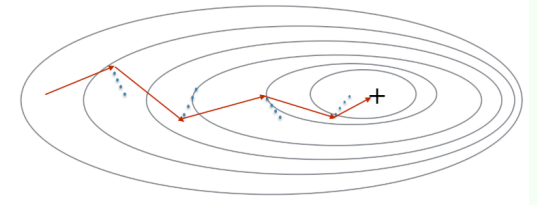
\includegraphics[width=70mm,scale=0.5]{images/nn_2_images/momentum.png}
                
                \caption*{The blue lines indicate the more "severe" path that we would've taken with normal gradient descent. the orange line is the line we take with momentum. }
            \end{figure}

            Notice that generally, the orange path is closer to correct! We still oscillate somewhat, but much less than we would have otherwise.

            \pagebreak

            
            

            

    \subsection{Adadelta}    

        \subsubsection{Per-weight step sizes}

            Earlier, we discussed creating \textbf{separate} step sizes for different weights in our network:
    
            \begin{itemize}
                \item Different weights could have different \gren{sensitivities}: one weight could have a much larger/smaller impact on $J$, based on \textbf{structure}.
    
                \item We already have the challenge of figuring out what \textbf{step sizes} cause \purp{slow convergence/divergence}: it would be even harder to find a step size that fit \textbf{all} of our weights, at the same time.
            \end{itemize}
    
            So, instead, we decided that each weight gets its \textbf{own step size}. 

            \begin{itemize}
                \item But, we never elaborated on \textbf{how} we compute that (adjustable) step size.\\
            \end{itemize}

            \begin{notation}
                Our base step size is indicated as $\eta$. 
                
                We'll call the \orgg{modified} step size for weight $j$, $\eta_j$.
            \end{notation}

        \phantom{}

        \subsubsection{Scaling}

            Our goal now, is to come up with a \orgg{systematic} way to \orgg{assign step sizes}. This allows us to \textbf{adjust}, rather than run our whole gradient descent with a "bad" step size.
                \note{So, we have less of a problem if we choose $\eta$ poorly.}

            Why do we adjust our step size? To avoid slow convergence, oscillation, or divergence.

            \begin{itemize}
                \item We might expect \purp{slow convergence} if the derivative is too \purp{small}: we carefully take small steps, but we aren't having much of an impact on $J$.

                    \begin{itemize}
                        \item Across this "flatter" region of the surface, in one direction, we might expect it to be safer to move further.
                    \end{itemize}

                \item We might expect \gren{divergence} or \gren{oscillation} if the derivative is too \gren{large}.
                    \begin{itemize}
                        \item We might end up "missing" possible solutions/local minima by \textbf{overshooting} them.
                        \item So, "steeper" regions might be riskier.
                    \end{itemize}
            \end{itemize}

            \begin{concept}
                Our goal is to \orgg{scale} our step size, so that it \textbf{adapts} to the situation:

                \begin{itemize}
                    \item We want to \purp{shrink} our step for \purp{large} gradients
                    \item We want to \gren{increase} our step for \gren{small} gradients
                \end{itemize}

                And we're interested in the \orgg{magnitude} of these gradients.
            \end{concept}


            This sort of behavior is easily captured by including a factor of $1/\norm{g_t}$. However, this has a smoothness problem: so, we'll use $1/\norm{g_t}^2$ instead.

            Though, we need to keep it separate for each of our data points.\\

            \begin{notation}
                The gradient for \vocab{weight $j$} at \redd{time $t$} is given as 

                \begin{equation*}
                    g_{\red{t},\blu{j}} = \nabla_W J(W_{\red{t-1}})_{\blu{j}}
                \end{equation*}

                Note the double-subscript.

                \phantom{}

                \begin{itemize}
                    \item By isolating weight $j$, we have a constant, not a vector.
                \end{itemize}
            \end{notation}

            We can now write our gradient update rule:

            \begin{equation}
                W_{\red{t},\blu{j}} \;\;=\;\; 
                W_{\red{t-1},\blu{j}} \;\;-\;\; 
                \eta_{\blu{j}} \cdot g_{\red{t},\blu{j}}
            \end{equation}

            And we're currently using the step size
                \note{Don't save this equation! It isn't our final formula.}

            \begin{equation}
                \eta_{\blu{j}} = \frac{\eta}{g_{\red{t},\blu{j}}^2}
            \end{equation}

        \phantom{}

        \subsubsection{Averaging}

            But, we don't necessarily know how "steep" our region \textbf{generally} is, based on the current gradient $g_t$. $g_t$ only gives us \textbf{one point} in space.
            
            It would be helpful to include information from the \textbf{past}: we'll be re-using the \textbf{weighted average}, once again.
                \note{Once again, it's helpful that the weighted average gradually "forgets" older information: we care less about gradients which are "further" from the present.}

            \begin{equation*}
                G_t \;\;=\;\; 
                \gamma G_{t-1} \;\;+\;\; 
                (1-\gamma) g_t^2 
                \qquad \qquad \text{(Maybe?)}
            \end{equation*}

            \begin{itemize}
                \item Note that we're averaging the \textbf{squared} magnitude.
            \end{itemize}
            
            Technically this is still \textbf{incorrect}: we need the $j$ notation.
                \note{It's incorrect because $g_t$ is a vector: we can't square it directly, we have to square its magnitude.}

            \begin{equation*}
                G_{\red{t},\blu{j}} \;\;=\;\; 
                \gamma G_{\red{t-1},\blu{j}} \;\;+\;\; 
                (1-\gamma) g_{\red{t},\blu{j}}^2 \qquad \qquad 
                \text{(Fixed!)}
            \end{equation*}

        \phantom{}

        \subsubsection{Division by zero}

            There's a problem with our weight adjustment:

            \begin{equation}
                \eta_j = \frac{\eta}{G_{\red{t},\blu{j}}}
            \end{equation}

            What happens if the denominator is near zero? It'll explode to a huge number! And at zero, it's undefined.

            To solve this, we'll add a very small constant, $\epsilon$.
                \note{We won't prescribe any particular choice of $\epsilon$ here.}

                \begin{equation}
                    \eta_j = \frac{\eta}{G_{\red{t},\blu{j}}+\epsilon}
                \end{equation}

            Now, our scaling factor will never be bigger than $1/\epsilon$.

        \phantom{}

        \subsubsection{Square root}

            One last concern, to wrap up: currently, we're diving by the \textbf{squared} gradient. This is actually somewhat overkill. 
            
            Remember that our goal is to do the following operation:

            \begin{equation}
                W_{\red{t},\blu{j}} = W_{\red{t-1},\blu{j}}  \;\;-\;\; 
                \underbrace{
                    \eta_{\blu{j}} \cdot g_{\red{t},\blu{j}}
                }_{\text{Update}}
            \end{equation}

            With our current formula, our update has 
            
            \begin{itemize}
                \item a factor of $g_{t,j}$ in the \textbf{numerator}
                \item from $\eta_j$, a factor proportional to $g_{t,j}^2$ in the \textbf{denominator} 
            \end{itemize}

            This is "scaling" our gradient by more than we want to. So, we'll take the \textbf{square root} of the denominator.
                \note{Our goal is to make the scales of different axes more similar, not to neglect dimensions with high gradient (high effect on loss)}

            \begin{equation}
                \eta_j = \frac{\eta}{ \sqrt{G_{\red{t},\blu{j}}+\epsilon} }
            \end{equation}

            This is the completed form of our \textbf{adadelta step size rule!}\\

            \begin{definition}
                \vocab{Adadelta} is a technique for \redd{adaptive step size}, which:

                \begin{itemize}
                    \item \purp{Decreases} step size in dimensions with a history of \purp{high-magnitude} gradients
                    \item \gren{Increases} step size in dimensions with a history of \gren{low-magnitude} gradients
                \end{itemize}

                Suppose our gradient for weight $W_j$ at time $t$ is represented by

                \begin{equation*}
                    g_{t,j} = \nabla_{W}J(W_{t-1})_j
                \end{equation*}

                    \phantom{}

                This is accomplished by \orgg{scaling} the step size $\eta$ to create $\eta_j$:

                \begin{equation*}
                    \eta_j = \frac{\eta}{ \sqrt{G_{\red{t},\blu{j}}+\epsilon} }
                \end{equation*}

                Where $G_{t,j}$ is a "\redd{running average}" of the previous gradients for weight $W_j$.

                \begin{equation*}  
                    \begin{gathered}
                        G_{\red{0},\blu{j}} = 0 \\
                        G_{\red{t},\blu{j}} \;\;=\;\; 
                        \gamma G_{\red{t-1},\blu{j}} \;\;+\;\;
                        (1-\gamma) g_{\red{t},\blu{j}}^2
                    \end{gathered}
                \end{equation*}

                So, our completed gradient descent rule takes the form:

                \begin{equation*}
                    W_{\red{t},\blu{j}} \;\;=\;\; 
                    W_{\red{t-1},\blu{j}}  \;\;-\;\; 
                    \frac{\eta}{ \sqrt{G_{\red{t},\blu{j}}+\epsilon} } \cdot g_{\red{t},\blu{j}}
                \end{equation*}
                
            \end{definition}

        \phantom{}

        \subsubsection{Sparse Data}

            One major advantage of adadelta is its use for \orgg{sparse datasets}, where many variables only show up in a small percentage of the data.

            \begin{itemize}
                \item If a variable is much less frequent, then the weighted average $G_t$ will be much smaller.
                \item So, when those data points \textbf{do} appear, the step size is much larger.
            \end{itemize}

            This allows our model to learn more from variables that don't show up as frequently.\\

            \begin{concept}
                \vocab{Adadelta} often works well with \purp{sparse data}: datasets where many variables rarely show up as non-zero.

                The step sizes for these variables become much larger, so our model can learn more from less-common information.
            \end{concept}

            However, this can run the risk of paying attention to variables that are sparse, but \textbf{not} especially meaningful. 
            
            \begin{itemize}
                \item It's important to choose your variables carefully, so the model doesn't "learn" from noise.
            \end{itemize}

        \phantom{}

        \subsection{Adagrad}

            Originally, adadelta derives from a \textbf{simpler} method, known as \vocab{adagrad}, or "adaptive gradient".

            \begin{itemize}
                \item The main difference with this approach is, rather than find the \textbf{weighted average} $G_t$, we simply \textbf{sum} the previous gradients.
            \end{itemize}

            The main problem with this approach is that, over time, $G_t$ becomes too \textbf{large}. So, our step size becomes too small, and our algorithm slows down.

            By averaging, we don't run into this problem of $G_t$ "accumulating": older data is gradually \textbf{forgotten}.

    \pagebreak
    \subsection{Adam}

        Momentum and Adadelta both bring some benefits:

        \begin{itemize}
            \item \purp{Momentum} averages our current gradient with \purp{previous gradients}, to reduce \textbf{oscillation} and make a more direct path to the solution.
            
            \item \gren{Adadelta} modifies our \gren{step sizes}: it takes smaller steps in directions of high gradient (reduce overshooting) and takes bigger steps in directions of low gradient (converge faster).
        \end{itemize}

        There's nothing structurally incompatible between them. So, why not incorporate both?

        \begin{itemize}
            \item This combination is called \vocab{Adam}: it has become the most popular way to handle step sizes in neural networks.\\
        \end{itemize}

        \begin{concept}
            \vocab{Adam} integrates the techniques of both \purp{momentum} and \gren{adadelta}.
        \end{concept}

        \phantom{}

        \subsubsection{Momentum and Adadelta}

            We used two different \textbf{running averages}, both using $\gamma$ for their "\textbf{discount factor}": how much we discount the effect of older data.
                \note{It's "discounting", or reducing the effect of older data, because $\gamma<1$.}
    
            \begin{itemize}
                \item We'll replace $\gamma$ with $B_1$ (momentum) and $B_2$ (adadelta).\\
            \end{itemize}

            \begin{notation}
                In the adam algorithm, $B_1$ and $B_2$ are \redd{discount factors} replacing $\gamma$ from momentum and adadelta.
            \end{notation}
    
            We use the same notation for gradients:
    
            \begin{equation}
                g_{t,j} = \nabla_W J(W_{t-1})_j
            \end{equation}
    
            First, we'll keep track of our\textbf{ averaged gradient}, $m_{t,j}$. This will be the \textbf{direction} we plan to move.

            \begin{equation}
                \blu{m_{t,j}} \;\;=\;\; 
                B_1 \blu{m_{t-1,j}} \;\;+\;\; 
                (1-B_1) \blu{ g_{t,j} }
            \end{equation}

            Then, we'll keep track of the \textbf{average squared gradient}, $v_{t,j}$. This will tell us whether to scale up/down our \textbf{step size} on each variable.

            \begin{equation}
                \red{v_{t,j}} \;\;=\;\; 
                B_2 \red{v_{t-1,j}} \;\;+\;\; 
                (1-B_2) \red{ g_{t,j}^2 }
            \end{equation}

            We can combine these into our equation, the way you use momentum and adadelta:

            \begin{equation}
                W_{t,j} \;\;=\;\; 
                W_{t-1,j}  \;\;-\;\; 
                \frac{\eta}{ \sqrt{\red{v_{t,j}}+\epsilon} } \cdot \blu{m_{t,j}}
            \end{equation}

            We're not quite done yet, though.

        \phantom{}

        \subsubsection{Normalization}

            There's one issue with our running average, that we should address.

            Suppose we have a sequence of numbers:

            \begin{equation}
                [1,1,1]
            \end{equation}

            What's the running average of this sequence of numbers, with $\gamma=.1$? You'd expect it to be 1 for all elements, right?

            \begin{itemize}
                \item We start with $a_0=0$.
            \end{itemize}

            \begin{equation}
                \begin{gathered}
                    a_1 = .1*0 + .9*1 = \org{.9} \\
                    a_2 = .1*.9+ .9*1 = \org{.99} \\
                    a_3 = .1*.99+ .9*1 = \org{.999}
                \end{gathered}
            \end{equation}

            It turns out not to be true! Why is that?

            Because of our initial term, $a_0$: it has nothing to do with the data. Because it'll always be 0, it \textbf{deflates} the value of all the remaining averages.

            How much does it deflate the average? Well, let's consider the general equation:

            \begin{equation}
                A_T = \sum_{t=0}^T \red{\gamma^{(T-t)}} \blu{(1-\gamma)^t} g_t
            \end{equation}

            What "fraction" of the total is missing, thanks to $A_0=0$? 
            
            \begin{itemize}
                \item Well, all of our weighted terms $\red{\gamma^{(T-t)}} \blu{(1-\gamma)^t}$ should add up to 1: each one represents the "percent/fraction" of the average which comes from that $g_t$ term.
            \end{itemize}

            $A_0$ matches $t=0$, so we find:

            \begin{equation}
                A_T = \overbrace{ A_0 \red{\gamma^T}}^{A_0=0} + 
                \sum_{t=1}^T \red{\gamma^{(T-t)}} \blu{(1-\gamma)^t} g_t
            \end{equation}

            So, out of our total $1$, or 100\%, we're missing $\gamma^T$.

            \begin{itemize}
                \item Our new total is $1-\gamma^T$.

                \item In order to correct for the "zeroed out" part of our average, we multiply by

                \begin{equation}
                    \frac{\text{Desired total}}{\text{Real total}}=\frac{1}{1-\gamma^T}
                \end{equation}
            \end{itemize}

            \begin{concept}
                We've chosen $A_0=0$: this is \orgg{unrelated} to our real data. 
                
                As a result, $A_t$ doesn't accurately reflect our weighted average: it's slightly \gren{smaller}.

                \begin{itemize}
                    \item $A_0$ is "included" as a 0, even though it's not a \redd{real} data point.
                    \item So, whatever \purp{percent} of our data is represented by $A_0$, is "falsely empty".
                \end{itemize}

                $A_0$ is scaled by $\red{\gamma^t}$, so that's the amount \purp{removed} from our "true" weighted average.

                The "real" weighted average, that ignores $A_0$, has to un-do the deflation caused by including fake, starting data:

                \begin{equation*}
                    \widehat{A}_t = A_t \cdot \frac{1}{1-\gamma^t}
                \end{equation*}
            \end{concept}

            We'll make this correction for our running averages:

            \begin{equation}
                \begin{gathered}
                    \widehat{m}_{t,j} = \frac{m_{t,j}}{1-B_1^t} \\
                    \widehat{v}_{t,j} = \frac{v_{t,j}}{1-B_2^t}
                \end{gathered}
            \end{equation}

        \phantom{}

        \subsubsection{Adam}

            Now, we have our complete equation for adam:\\

            \begin{definition}
                \vocab{Adam} is a technique for improving \orgg{gradient descent} that integrates two other techniques. Our computed gradient is given as 

                \begin{equation*}
                    g_{t,j} = \nabla_{W}J(W_{t-1})_j
                \end{equation*}

                \begin{itemize}
                    \item \purp{Momentum} averages our previous gradients with our current one, to reduce oscillation and get a "averaged" view of data. $B_1$ gives the weight of old data.

                        \begin{equation*}
                            \begin{gathered}
                                m_{0,j} = 0 \qquad \qquad
                            \blu{m_{t,j}} \;=\; B_1 \blu{m_{t-1,j}} \;+\; (1-B_1) \blu{ g_{t,j} }
                            \end{gathered}
                        \end{equation*}

                    \item \gren{Adadelta} estimates how "steep" our gradient has been recently, and uses it to adjust our step size, for better convergence. $B_2$ gives the weight of old data.

                            \begin{equation*}
                                \begin{gathered}
                                    v_{0,j} = 0 \qquad \qquad
                                    \red{v_{t,j}} \;=\; B_2 \red{m_{t-1,j}} \;+\; (1-B_2) \red{ g_{t,j}^2 }
                                \end{gathered}
                            \end{equation*}
                        \end{itemize}

                We include a \textbf{correction} factor for the zeroed initial conditions: $m_0=v_0=0$.

                \begin{equation*}
                    \widehat{\blu{m}}_{t,j} = \frac{\blu{m}_{t,j}}{1-B_1^t}
                    \qquad \qquad 
                    \widehat{\red{v}}_{t,j} = \frac{\red{v}_{t,j}}{1-B_2^t}
                \end{equation*}

                Finally, our update rule takes the form:

                \begin{equation*}
                    W_{t,j} = W_{t-1,j}  
                        \;\;-\;\; 
                    \frac{\eta}{ \sqrt{\red{\widehat{v}_{t,j}}+\epsilon} } \cdot \blu{\widehat{m}_{t,j}}
                \end{equation*}
            \end{definition}

            Impressively, adam is not very sensitive to the initial conditions for $\epsilon$, $B_1$ and $B_2$.
                \note{It's able to "self-correct" its step sizes and gradient based on data.}

            To implement this for NNs, we just need to keep track of each value, for each weight. If you do it systematically, this is easier than it sounds.

\pagebreak

\section{Batch Normalization Details}

    Let's review the general premise 
    
    of batch normalization:\\

    \begin{definition}
            \vocab{Batch Normalization} is a process where we

            \begin{itemize}
                \item Standardize the pre-activation for each layer using the mean $\mu_i$ and standard deviation $\sigma_i$ (for the $\nth{i}$ dimension). Select $\epsilon$: $0 < \epsilon<<1$.

                \begin{equation*}
                    \red{ \overline{Z}_{ij} } =  \frac{ \red{Z_{ij}}  -\blu{\mu_i}}{\sigma_i+\epsilon}
                \end{equation*}
                
                \item Choose the new mean and standard deviation for the pre-activation using $(n \times 1)$ vectors $G$ and $B$

                \begin{equation*}
                    \red{\widehat{Z}_{ik}} = \pur{G_i} * \red{\overline{Z}_{ij}} + \grn{B_i}
                \end{equation*}
            \end{itemize}
            
        \end{definition}


        \subsection{Applying batch normalization to backprop} 

            \phantom{}

            \begin{remark*}
                The following section mostly deals with the details of computing batch normalization derivatives.
            \end{remark*}

            As we showed with our figure,

            \begin{figure}[H]
                \centering
                    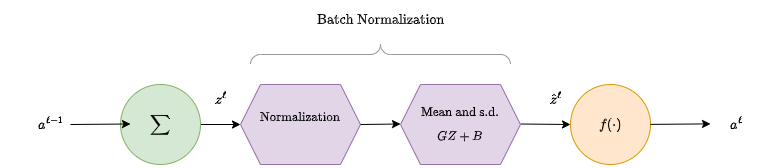
\includegraphics[width=120mm,scale=0.5]{images/nn_2_images/batch_normalization.png}
            \end{figure}

            Batch normalization adds two units that \textbf{interrupt} our chain of nested functions.

            That means we need to figure out how to do backprop, bridging across the new gap between \blu{$Z$} and \red{$\widehat{Z}$}.


            So, that only leaves a couple problems:

            \begin{itemize}
                \item "Bridging the gap" between derivatives before and after BN, with $\pderivslash{\red{\widehat{Z}^\ell}}{\blu{Z^\ell}}$.
                
                \item Gradients for \gren{$G$} and \purp{$B$}: they're parameters now, too, so we need to train them.\\
                
            \end{itemize}

            \begin{concept}
                Introducing batch normalization add new functions \purp{in between} our old ones. 

                \begin{itemize}
                    \item Our input data has to travel through those additional layers.
                    \item This \orgg{changes} the relationship between our current value, and the output loss.
                \end{itemize}

                So, in order to do backprop correctly, we have to figure out the \gren{derivatives} of those functions.
            \end{concept}


        \subsubsection{Bridging the gap}

            We want to connect the start and end of batch normalization:\\

            \begin{equation}
                \pderiv{\red{\widehat{Z}}}{\blu{Z}}
            \end{equation}

            As usual, with the chain rule, we'll connect them by considering any values/function \textbf{between} them.

            In this case, $Z$ is normalized ($\overline{Z}$), and \textbf{then} we apply $G$ and $B$ ($\widehat{Z}$). We're missing the "normalized" step.

            \begin{equation}
                \pderiv{\red{\widehat{Z}}}{\blu{Z}} = 
                \pderiv{\red{\widehat{Z}}}{\grn{\overline{Z}}} \cdot \pderiv{\grn{\overline{Z}}}{\blu{Z}}
            \end{equation}

            Let's compare any two of these : $\red{\widehat{Z}}$ and $\grn{\overline{Z}}$, for example.

            \begin{itemize}
                \item These are both $(n \times k)$ matrices.
                \item That means that each has two dimensions of variables. If we were to take the derivative between them, we would need $2*2$ axes: a \purp{4-tensor}.
            \end{itemize}

            That sounds terrible. Instead, we'll compute these derivatives \textbf{element-wise}.

            \begin{equation}
                \pderiv{ \red{\widehat{Z}_{ab}} }{ \blu{Z_{ef}} } = 
                \pderiv{ \red{\widehat{Z}_{ab}} }{ \grn{\overline{Z}_{cd} } } \cdot 
                \pderiv{ \grn{\overline{Z}_{cd}} }{ \blu{Z_{ef}} }
            \end{equation}

            \subsecdiv

        \subsubsection{Indexing}

            First, let's simplify these indices: only some pairs of elements matter.

            \begin{equation}
                \red{\widehat{Z}_{ik}} = G_i * \grn{\overline{Z}_{ik}} + B_i
            \end{equation}

            It seems that $\red{\widehat{Z}_{ik}}$ is only affected by the element with the same indices: $\grn{\overline{Z}_{ik}}$.\\

            \begin{concept}
                $\red{\widehat{Z}_{ik}}$  is only a function of the same index element $\grn{\overline{Z}_{ik}}$.

                \begin{itemize}
                    \item Any other elements from $\grn{\overline{Z}}$ has no effect.
                \end{itemize}

                \begin{equation*}
                    (\red{a} \neq \grn{c} \text{ or } \red{b} \neq \grn{d}) \implies 
                    \pderiv{ \red{\widehat{Z}_{ab}} }{ \grn{\overline{Z}_{cd} } }=0
                \end{equation*}

                So, we write our remaining derivatives as $\pderivslash{ \red{\widehat{Z}_{ik}} }{ \grn{\overline{Z}_{ik} } }$.
            \end{concept}
        

            What about the other derivative?

            \begin{equation*}
                \grn{ \overline{Z}_{ik} } =  \frac{ \blu{Z_{ik}}  -\blu{\mu_i}}{ \blu{\sigma_i}+\epsilon}
            \end{equation*}

            $\mu_i$ and $\sigma_i$ include various different data points $\blu{Z_{ik}}$, but only the $\nth{i}$ dimension. $\blu{Z_{ik}}$ requires the exact same indices.\\

            \begin{concept}
                $\grn{\overline{Z}_{ik}}$ is only a function of elements in the same dimension $i$, $\blu{Z_{ij}}$.

                \begin{equation*}
                    \grn{c} \neq \blu{e} \implies \pderiv{ \grn{\overline{Z}_{cd}} }{ \blu{Z_{ef}} } = 0
                \end{equation*}

                Our remaining derivatives take the form $\pderivslash{ \grn{\overline{Z}_{ik}} }{ \blu{Z_{ij}} }$.
            \end{concept}

            If we boil this down, we get all of our non-zero derivatives:

            \begin{equation}
                \pderiv{ \red{\widehat{Z}_{ik}} }{ \blu{Z_{ij}} } = 
                \pderiv{ \red{\widehat{Z}_{ik}} }{ \grn{\overline{Z}_{ik} } } \cdot 
                \pderiv{ \grn{\overline{Z}_{ik}} }{ \blu{Z_{ij}} }
            \end{equation}

        \subsubsection{Computing $\pderivslash{ \red{\widehat{Z}_{ik}} }{ \grn{\overline{Z}_{ik} } }$}

            We return to our previous equation:

            \begin{equation}
                \red{\widehat{Z}_{ik}} = G_i * \grn{\overline{Z}_{ik}} + B_i
                \quad \implies \quad
                \pderiv{ \red{\widehat{Z}_{ik}} }{ \grn{\overline{Z}_{ik} } } = G_i
            \end{equation}

        \subsubsection{Computing $\pderivslash{\grn{\overline{Z}_{ik}}}{\blu{Z_{ij}}}$}

            For the other derivative:

            \begin{equation}
                \grn{\overline{Z}_{ik}}  =  \frac{ \org{Z_{ik} }  - \org{\mu_i}}{\org{\sigma_i}+\epsilon}
            \end{equation}

            This gets a bit complicated, because $\blu{Z_{ij}}$ can affect three different terms: $\org{Z_{ik}}$, $\org{\mu_i}$, and $\org{\sigma_i}$. 

            We'll solve this by using the multi-variable chain rule.
                \note{We're linearly adding the effect due to each of these three variables, separately.}

            \begin{equation}
                \pderiv{\grn{\overline{Z}_{ik}}}{\blu{Z_{ij}}} 
                \;\;=\;\;
                \overbrace{
                    \pderiv{\grn{\overline{Z}}_{ik}}{\org{Z_{ik}}} \cdot 
                    \deriv{\org{Z_{ik}}}{\blu{Z_{ij}}}
                }^{\text{$\org{Z_{ik}}$'s effect}}
                \;\;+\;\;
                \overbrace{
                    \pderiv{\grn{\overline{Z}}_{ik}}{\org{\mu_i}} \cdot 
                    \deriv{\org{\mu_i}}{\blu{Z_{ij}}}
                }^{\text{$\org{\mu_i}$'s effect}}
                \;\;+\;\;
                \overbrace{
                    \pderiv{\grn{\overline{Z}}_{ik}}{\org{\sigma_i}} \cdot 
                    \deriv{\org{\sigma_i}}{\blu{Z_{ij}}}
                }^{\text{$\org{\sigma_i}$'s effect}}
            \end{equation}

            In each of these terms, we treat the other two variables as "constant".

        \subsubsection{Lots of mini-derivatives}

            Let's compute the $\grn{\overline{Z}}$ derivatives.

            \begin{equation}
                \grn{\overline{Z}_{ik}}  =  \frac{ Z_{ik}   - \mu_i}{\sigma_i+\epsilon}
            \end{equation}

            gives us

            \begin{equation}
                \pderiv{\grn{\overline{Z}}_{ik}}{\org{Z_{ik}}} = 
                \frac{1}{\sigma_i+\epsilon}
                    \qquad \qquad
                \pderiv{\grn{\overline{Z}}_{ik}}{\org{\mu_i}} = 
                \frac{-1}{\sigma_i+\epsilon}
                    \qquad \qquad
                \pderiv{\grn{\overline{Z}}_{ik}}{\org{\sigma_i}} = 
                -\Big( 
                    \frac{ Z_{ik}-\mu_i  }{(\sigma_i+\epsilon)^2}
                \Big)
            \end{equation}

            Now, let's compute the $\blu{Z_{ij}}$ derivatives.

            \begin{equation}
                \boxed{\pderiv{\org{Z_{ik}}}{\blu{Z_{ij}}} = \delta_{jk}} 
                =
                \mathbf{1}(j=k) = 
                \begin{cases}
                    1 & j=k \\
                    0 & j \neq k
                \end{cases}
            \end{equation}

            \begin{equation}
                \org{\mu_i} =\frac{1}{K} \sum_{j=1}^K \blu{Z_{ij}} 
                    \implies 
                \boxed{\pderiv{ \org{\mu_i} }{ \blu{Z_{ij}} } = \frac{1}{K}}
            \end{equation}

            \begin{equation}
                \org{\sigma^2_i} = \frac{1}{K} \sum_{j=1}^K (\blu{Z_{ij}}-\mu_i)^2  
                    \implies 
                \boxed{\pderiv{ \org{\sigma_i} }{ \blu{Z_{ij}} } = \frac{\blu{Z_{ij}}-\mu_i}{K\sigma_i}}
            \end{equation}

            

            
        \subsubsection{Assembling our derivatives}

            Now, we plug them in.

            \begin{equation}
                \pderiv{\grn{\overline{Z}_{ik}}}{\blu{Z_{ij}}} =
                \pderiv{\grn{\overline{Z}}_{ik}}{\org{Z_{ik}}} \cdot 
                \deriv{\org{Z_{ik}}}{\blu{Z_{ij}}}
                +
                \pderiv{\grn{\overline{Z}}_{ik}}{\org{\mu_i}} \cdot 
                \deriv{\org{\mu_i}}{\blu{Z_{ij}}}
                +
                \pderiv{\grn{\overline{Z}}_{ik}}{\org{\sigma_i}} \cdot 
                \deriv{\org{\sigma_i}}{\blu{Z_{ij}}}
            \end{equation}

            First, the $\grn{\overline{Z}}$ derivatives.

            \begin{equation}
                \pderiv{\grn{\overline{Z}_{ik}}}{\blu{Z_{ij}}} =
                \Big( \frac{1}{\sigma_i+\epsilon} \Big) \cdot 
                \deriv{\org{Z_{ik}}}{\blu{Z_{ij}}}
                -
                \Big( \frac{1}{\sigma_i+\epsilon} \Big) \cdot 
                \deriv{\org{\mu_i}}{\blu{Z_{ij}}}
                -
                \Big( 
                    \frac{ Z_{ik}-\mu_i  }{(\sigma_i+\epsilon)^2}
                \Big) \cdot 
                \deriv{\org{\sigma_i}}{\blu{Z_{ij}}}
            \end{equation}

            And now the $\blu{Z_{ij}}$ derivatives.

            \begin{equation}
                \pderiv{\grn{\overline{Z}_{ik}}}{\blu{Z_{ij}}} =
                \Big( \frac{1}{\sigma_i+\epsilon} \Big) \cdot 
                \delta_{jk}
                -
                \Big( \frac{1}{\sigma_i+\epsilon} \Big) \cdot 
                \Big( \frac{1}{K} \Big)
                -
                \Big( 
                    \frac{ Z_{ik}-\mu_i  }{(\sigma_i+\epsilon)^2}
                \Big) \cdot 
                \Big( \frac{\blu{Z_{ij}}-\mu_i}{K\sigma_i} \Big)
            \end{equation}

            \begin{kequation}
                We have found the batch normalization derivatives

                \begin{equation*}
                    \pderiv{ \red{\widehat{Z}_{ik}} }{ \grn{\overline{Z}_{ik} } } = G_i
                \end{equation*}

                \begin{equation*}
                    \pderiv{\grn{\overline{Z}_{ik}}}{\blu{Z_{ij}}} =
                    \frac{1}{K(\sigma_i+\epsilon)}
                    \Big( K \delta_{jk} - 1 - \frac{(Z_{ik}-\mu_i)(Z_{ij}-\mu_i)}{\sigma_i(\sigma_i+\epsilon)} \Big)
                \end{equation*}

                Which we multiply together to find $\pderivslash{ \red{\widehat{Z}_{ik}} }{ \blu{Z_{ij}} }$.
            \end{kequation}

            Once we've computed these derivatives, we can use them to extend the chain of $\pderivslash{L}{\red{\widehat{Z}_{ik}} }$. 

            We're aiming to handle both of the batch normalization functions, with $\pderivslash{L}{\blu{Z_{ij}}}$. 
                \note{We're going from $\red{\widehat{Z}_{ik}}$, which is post-BN, to $\blu{Z_{ij}}$, which is pre-BN. }

            \begin{itemize}
                \item $\blu{Z_{ij}}$ affects every data point $\red{\widehat{Z}_{ik}}$, and every data point affects $L$.
                \item So, we'll have to consider every data point $k$ using the multi-variable chain rule:
            \end{itemize}
            

            \begin{equation}
                \pderiv{L}{\blu{Z_{ij}}} = 
                \underbrace{ \sum_{k=1}^K }_{\text{MV Chain Rule}}
                \overbrace{
                    \pderiv{L}{\red{\widehat{Z}_{ik}} } \cdot 
                    \pderiv{ \red{\widehat{Z}_{ik}} }{ \blu{Z_{ij}} }
                }^{\text{Data point $k$'s effect}}
            \end{equation}

            We can use this to go further back in our layers: as far as we want, as long as we don't forget this derivative!
            

        \subsubsection{Gradients for $B$ and $G$}

            We want $\pderivslash{L}{\org{B}}$ and $\pderivslash{L}{\pur{G}}$. Thanks to the work we did just now, we can travel backwards through numberous layers, to reach any $B^\ell$ and $G^\ell$. 

            So, we'll assume we have $\pderivslash{L}{\widehat{Z^\ell}}$. Once again, we'll omit the layer notation.

            \begin{itemize}
                \item We'll focus on a single bias, $B_i$: this biases one dimension of $\red{\widehat{Z}_{ik}}$.

                \begin{equation}
                    \red{\widehat{Z}_{ik}} = \pur{G_i} * \grn{\overline{Z}_{ik}} + \org{B_i}
                    \quad \implies \quad
                    \pderiv{ \red{\widehat{Z}_{ik}} }{ \org{B_i} }  = 1
                \end{equation}
                
                \item This bias is applied to every of our $K$ data points: every data point affects the loss $L$. So, we'll have to sum them with the multi-variable chain rule.
            \end{itemize}

            This is exactly the same as how we did $\pderivslash{L}{\blu{Z_{ij}}}$.

            \begin{equation}
                \pderiv{L}{\org{B_i}} = 
                \sum_{k=1}^K 
                \pderiv{L}{ \red{\widehat{Z}_{ik}} } \cdot \pderiv{\red{\widehat{Z}_{ik}}}{\org{B_i}} =
                \boxed{
                \sum_{k=1}^K 
                \pderiv{L}{ \red{\widehat{Z}_{ik}} }
                }
            \end{equation}

            Now, we focus on a single scaling factor $G_i$: 

            \begin{equation}
                \red{\widehat{Z}_{ik}} = \pur{G_i} * \grn{\overline{Z}_{ik}} + \org{B_i}
                \quad \implies \quad
                \pderiv{ \red{\widehat{Z}_{ik}} }{ \pur{G_i}  }  = \grn{\overline{Z}_{ik}}
            \end{equation}

            And once again, we add across different data points:

            \begin{equation}
                \pderiv{ L }{ \pur{G_i}  } = 
                \sum_{k=1}^K 
                \pderiv{L}{ \red{\widehat{Z}_{ik}} } \cdot \pderiv{\red{\widehat{Z}_{ik}}}{\pur{G_i}} =
                \boxed{
                    \sum_{k=1}^K 
                    \pderiv{L}{ \red{\widehat{Z}_{ik}} } \grn{\overline{Z}_{ik}}
                }
            \end{equation}


        We're finished.\\

        \begin{kequation}
            Here, we have the gradients for the batch scaling coefficients, $B$ and $G$.

            \begin{equation*}
                \pderiv{L}{\org{B_i}} =
                \sum_{k=1}^K 
                \pderiv{L}{ \red{\widehat{Z}_{ik}} }
            \end{equation*}

            \begin{equation*}
                \pderiv{ L }{ \pur{G_i}  } =
                \sum_{k=1}^K 
                \pderiv{L}{ \red{\widehat{Z}_{ik}} } \grn{\overline{Z}_{ik}}
            \end{equation*}
        \end{kequation}